%------------------------------------------------------------------------
%Editar Diplomado
\hypertarget{cv:GestionarProyectosAdmin}{\section{Gestionar Proyectos de Administrador}} \label{sec:GestionarProyectosAdmin}

	Esta funcionalidad le permitirá las acciones necesarias para controlar los proyectos que han sido previamente registrados en el sistema, como lo son visualizar el listado de los proyectos, registrar un nuevo proyecto, modificar uno existente o eliminarlo.

		\subsection{Procedimiento}

			%Pasos de procedimiento
			\begin{enumerate}
	
			\item Seleccione la opción \textbf{Proyectos} del menú \ref{fig:MN-AD}.
	
			\item Se mostrará la pantalla \ref{fig:GestionarProyectosAdmin} ''Gestionar Proyectos de Administrador''.

			%Pantalla
			\begin{figure}[htbp!]
				\begin{center}
					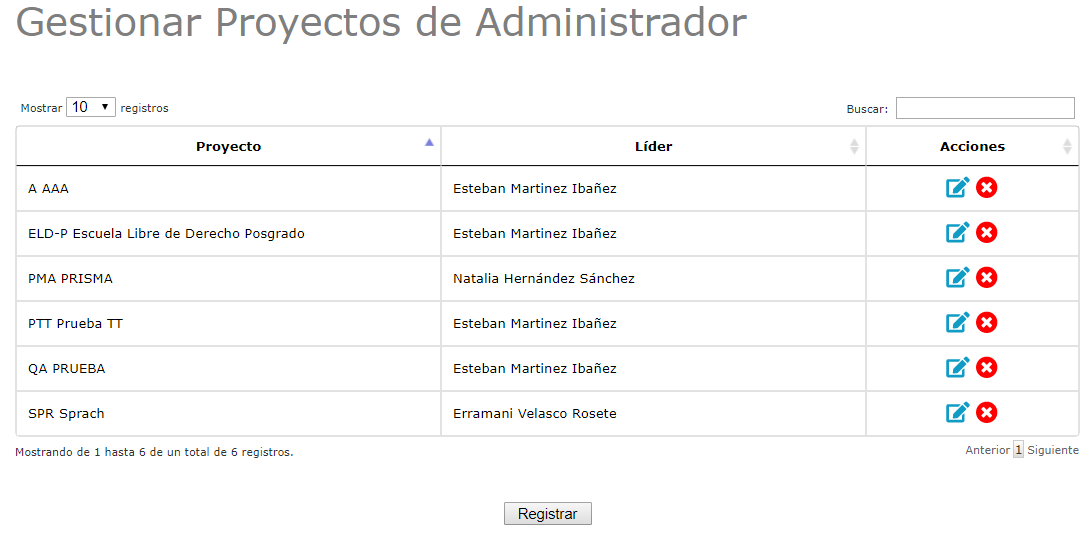
\includegraphics[scale=0.6]{roles/administrador/proyectosAdmin/gestionarproyectosAdmin/pantallas/IU2GestionProyectos}
					\caption{Gestionar Proyectos de Administrador}
					\label{fig:GestionarProyectosAdmin}
				\end{center}
			\end{figure}
		
				\item Seleccione la operación que desea realizar:
			
			Para (\hyperlink{cv:registrarProyectoAdmin}{Registrar}) dé clic en el botón \IURegistrar.
			
			Para (\hyperlink{cv:modificarProyecto}{Modificar}) dé clic en el icono \IUEditar{} de algún proyecto ya registrado.
			
			Para (\hyperlink{cv:eliminarProyecto}{Eliminar}) dé clic en el icono \IUBotonEliminar{} de algún proyecto ya registrado.
			
			
			\end{enumerate}